% =====================================================================
%  SchemaLens-Cassandra (TSDB / IoT) -- Relatorio metodologico completo
%  Compilar no Overleaf com pdfLaTeX. Figuras em figs/ (PDF).
% =====================================================================
\documentclass[11pt,a4paper]{article}

\usepackage[T1]{fontenc}
\usepackage[utf8]{inputenc}
\usepackage{lmodern}
\IfFileExists{brazil.ldf}{\usepackage[brazil]{babel}}{}
\usepackage[a4paper,margin=2.3cm]{geometry}
\usepackage{amsmath,amssymb}
\usepackage{graphicx}
\usepackage{booktabs,tabularx,longtable,array}
\usepackage{float}
\usepackage[font=small,labelfont=bf]{caption}
\usepackage[table]{xcolor}
\usepackage{microtype}
\usepackage{listings}
\usepackage{fancyhdr}
\usepackage[colorlinks=true,linkcolor=blue!50!black,urlcolor=blue!50!black,citecolor=green!40!black]{hyperref}

\definecolor{boxbg}{RGB}{243,246,250}
\definecolor{warnbg}{RGB}{253,244,232}
\newcommand{\caixa}[2][boxbg]{\par\smallskip\noindent\colorbox{#1}{\parbox{\dimexpr\linewidth-2\fboxsep}{#2}}\par\smallskip}
\newcommand{\just}[1]{\caixa{\textbf{Justificativa.} #1}}
\newcommand{\limit}[1]{\caixa[warnbg]{\textbf{Limitação.} #1}}
\newcolumntype{Y}{>{\raggedright\arraybackslash}X}

\lstset{basicstyle=\ttfamily\footnotesize,columns=fullflexible,frame=single,
        backgroundcolor=\color{boxbg},breaklines=true,showstringspaces=false,
        keywordstyle=\bfseries\color{blue!50!black},language=SQL}

\pagestyle{fancy}\fancyhf{}
\lhead{\small SchemaLens--Cassandra (TSDB/IoT)}\rhead{\small Relatório metodológico}
\cfoot{\thepage}

\title{\textbf{SchemaLens--Cassandra para séries temporais IoT}\\[4pt]
\large Reconstrução metodológica completa, do catálogo TS0--TS8 aos resultados das Fases 2--4,\\
com justificativas, leitura crítica e o que pode ser ajustado ou concluído}
\author{Projeto \texttt{SchemaLens\_IoT\_Cassandra\_V3\_Automatico}}
\date{Período coberto: 16/10/2026 a 12/11/2026 \quad--\quad documento gerado em 13/11/2026}

\begin{document}
\maketitle

\begin{abstract}
\noindent Este documento reconstrói, a partir dos artefatos efetivamente presentes no repositório (manifestos, CSVs auditados, protocolos, emendas e relatórios), tudo o que foi feito na adaptação da metodologia SchemaLens para o Apache Cassandra com cargas de séries temporais do \emph{IoT Benchmark}. O SchemaLens propõe gerar, \emph{antes de qualquer medição}, um conjunto pequeno e explicável de projetos físicos candidatos a partir de evidências do workload. Descrevemos cada estágio (ativação de famílias, instanciação física, planos de consulta e escrita, proxies analíticos, seleção HBench por Pareto, execução com oráculo semântico) e cada revisão (V3, V4, Rev2, Rev3), justificando as decisões. Em seguida explicamos \emph{por que} os experimentos recentes comparam apenas dois candidatos --- TS2-U (tabela larga sem bucket) e TS2-D (tabela larga com bucket diário) ---, apresentamos os resultados de S1--S3 e das Fases 2--4 (mais de 40 mil latências auditadas, holdouts com dados Java novos, preditores Rev4/Rev5 e a regra T5) e encerramos com o que já pode ser concluído e o que precisa ser ajustado. A principal conclusão é dupla: (i) a cadeia SchemaLens funcionou como mecanismo \emph{auditável e explicável} de redução do espaço de projeto e previu exatamente o trabalho estrutural de cada consulta; (ii) neste workload estreito, o candidato vencedor (TS2-U) é fisicamente idêntico à tradução direta do modelo \texttt{table} do IoTDB, de modo que \emph{ainda não há evidência de ganho de desempenho sobre a referência}; essa evidência exige workloads que ativem mais famílias.
\end{abstract}

\tableofcontents
\newpage

% =====================================================================
\section{Resumo executivo: as respostas curtas}
% =====================================================================

\begin{enumerate}
\item \textbf{O que é o SchemaLens aqui.} Um pipeline em nove estágios que transforma \emph{workload + dados} em um conjunto pequeno de \emph{deployments} físicos Cassandra (HBench), congelado por hash \emph{antes} de qualquer medição, com uma explicação registrada para cada escolha. Medições servem para \emph{avaliar} o método, nunca para retroalimentar a seleção da mesma campanha (``firewall científico'').
\item \textbf{O que foi construído.} Stages 1--8 automáticos sobre dados e objetos de consulta gerados pelo código Java oficial do IoT Benchmark (commit \texttt{62e0dc10}); executor Stage 9 com oráculo semântico; quatro revisões do seletor (V3, V4-Auto, Rev2, Rev3 \emph{plan-aware}); dois holdouts confirmatórios (A e B); e uma sequência de experimentos de sensibilidade (S1, S2, S3, Fases 2, 3 e 4).
\item \textbf{Por que só restaram dois candidatos.} Porque o workload do IoT Benchmark nesta configuração é estreito (um dispositivo por consulta, dois sensores DOUBLE alinhados, leituras por intervalo): só 5 das 9 famílias ativam; TS1 é dominada por TS2; TS5 é inelegível (janelas não alinhadas); TS4 passou a ser dominada quando Q8 ganhou um plano de leitura descendente; TS0 ficou fora do Pareto e perdeu nas medições. A única decisão física que permaneceu aberta foi o modificador \textbf{M1 (granularidade do bucket)}: \emph{com} bucket diário (TS2-D) ou \emph{sem} bucket (TS2-U). Os estudos S1--Fase 4 foram desenhados para responder só essa pergunta (Seção~\ref{sec:doiscand}).
\item \textbf{Quem ganha e por quê.} TS2-U vence em cerca de 75--80\% dos casos temporais em todos os cenários testados (densidade 1--8$\times$, histórico de 21 a 333 dias, 3 a 18 dispositivos, partições de até 17\,MB, SSTable ou memtable, cache quente ou parcialmente frio). O mecanismo é explicável: cada chamada CQL tem custo fixo ($\approx$0,5--0,7\,ms no cliente), e TS2-D precisa de uma chamada por dia da janela; em janelas longas (80 e 330 dias) TS2-D perdeu 12 de 12 casos, com mediana D/U = 2,06.
\item \textbf{O que não deu certo.} Nenhum preditor pré-benchmark (Rev4 log-linear, Rev5 aditivo, regra T5 com zona de empate) superou a regra trivial ``sempre U''. A regra T5 foi testada de forma confirmatória e \emph{rejeitada} nas quatro hipóteses pré-registradas --- um resultado negativo honesto.
\item \textbf{Ponto crítico.} TS2-U tem exatamente o mesmo DDL da tabela de referência (tradução Cassandra do modelo \texttt{table} do IoTDB). Logo, nesta carga, o SchemaLens \emph{convergiu para o projeto de referência}; não produziu um esquema mais rápido do que ele. O valor demonstrado é de \emph{redução explicável e auditável}, não de ganho de desempenho.
\end{enumerate}

% =====================================================================
\section{Objetivo, pergunta de pesquisa e princípios}
% =====================================================================

\subsection{Pergunta}
O SchemaLens (originalmente validado em bancos de documentos/MongoDB) busca reduzir, \emph{antes do benchmarking}, o número de esquemas físicos que merecem ser materializados e medidos, preservando as alternativas promissoras e produzindo \emph{explicações técnicas} para ativar ou descartar cada uma. A extensão estudada aqui aplica a ideia ao Cassandra com séries temporais: as decisões relevantes são chave de partição, chave de \emph{clustering}, \emph{bucketing} temporal, colocalização de métricas e estruturas derivadas (último valor, \emph{rollups}).

Formalmente, o pipeline é
\[
\underbrace{A(q)=\alpha(M_q, G_{TS})}_{\text{ativação}} \;\to\; P \;\to\; C \;\to\; H \;\to\; H_{\text{bench}} \;\to\; \text{medições},
\]
em que $A(q)$ são as famílias ativadas pela evidência da consulta $q$, $P$ os planos, $C$ os custos analíticos, $H$ as configurações completas válidas e $H_{\text{bench}}$ o subconjunto congelado para medição.

\subsection{Princípios metodológicos adotados (e por quê)}
\begin{description}
\item[Firewall científico.] Nenhuma latência medida, vencedor de benchmark ou ID de consulta pode entrar na ativação ou na pré-seleção (\texttt{benchmark\_metrics\_allowed\_for\_selection=false}). \emph{Justificativa:} se a seleção usa o resultado que depois a avalia, a avaliação é circular (vazamento de informação, \emph{data leakage}).
\item[Congelamento por hash.] Stage 8 grava SHA-256 de entradas, regras, código e seleção; o executor recusa rodar se algo mudou. \emph{Justificativa:} torna verificável que a seleção antecedeu a medição.
\item[Pré-registro e emendas.] Desde a Rev2, hipóteses, sementes, rodadas e critérios são gravados \emph{antes} de medir; mudanças viram emendas datadas (EMENDA\_01 a 05). \emph{Justificativa:} prática de pré-registro~\cite{nosek2018}, que separa análise confirmatória de exploratória.
\item[Oráculo semântico.] Toda resposta de toda variante é comparada com um avaliador lógico independente do layout físico, antes e durante a medição (fora da região cronometrada). \emph{Justificativa:} só faz sentido comparar latência de projetos que devolvem a mesma resposta.
\item[Segurança operacional.] Somente keyspaces novos, \texttt{CREATE} sem \texttt{IF NOT EXISTS}, nenhum \texttt{DROP/TRUNCATE/ALTER}; evidência gravada em modo exclusivo (sem sobrescrita); medição interrompida é descartada inteira e refeita (EMENDA\_02).
\end{description}

% =====================================================================
\section{Linha do tempo do repositório}
% =====================================================================

\begin{longtable}{@{}p{1.6cm}p{6.3cm}p{6.6cm}@{}}
\toprule
\textbf{Data} & \textbf{Marco} & \textbf{Onde está} \\ \midrule
\endhead
antes de 16/10 & Catálogo TS0--TS8 e motor de regras herdados do SchemaLens TSBS/SmartRetail; fase A1 (ponte IoT, fixture); Piloto 1 e Rev2 do Stage 4 (divisão TS2-D/TS2-U) & \texttt{phase\_a1/vendor}, \texttt{archive/}, \texttt{docs/REV2\_STAGE4\_GRANULARIDADE\_PT.md} \\
16/10 & V3 automática: geração Java + captura dos 12 objetos de consulta + Stages 1--8; correção Q12; primeiro Stage 9 e referência nativa & \texttt{run\_v3\_auto.sh}, \texttt{native\_auto\_work/runs/} \\
26/10 & Diagnósticos E1--E3; V4 (fonte canônica + cobertura cruzada, E4); V4-Auto; V4 Rev2 (custos novos) e holdout Java independente; correções GROUP\_BY e teste TS5 & \texttt{SchemaLens\_Diagnostics\_V3\_E1\_E2\_E3}, \texttt{SchemaLens\_V4\_*} \\
04--05/11 & Auditoria Stage 7/8 da Rev2; armazenamento físico; telemetria TS0; E5 (Q8 TS0); Rev3 \emph{plan-aware}; campanhas confirmatórias A e B; S1 & \texttt{SchemaLens\_Rev2\_*}, \texttt{SchemaLens\_Rev3\_*} \\
05/11 & S2 (densidade 1--8$\times$) & \texttt{experiments/rev3\_s2\_partition\_growth} \\
10/11 & S3 R1 (estado físico controlado, SSTable) & \texttt{experiments/rev3\_s3\_physical\_storage} \\
11/11 & Fase 2 (E0--E6): réplicas, Rev4, histórico real, dispositivos, cache frio & \texttt{experiments/rev3\_fase2} \\
12/11 & Fase 3 (E7--E12) e Fase 4 (E13--E18): Rev5, holdout E9, tracing, regra T5 & \texttt{experiments/rev3\_fase2}, \texttt{SchemaLens\_Rev3\_Fase3\_Fase4\_results.zip} \\
\bottomrule
\end{longtable}

% =====================================================================
\section{O pipeline, estágio por estágio}
% =====================================================================

\subsection{Entradas: dados e workload do IoT Benchmark}
\paragraph{O que foi feito.} O repositório oficial \texttt{thulab/iot-benchmark}~\cite{iotbench,iotbenchpaper} foi clonado e fixado no commit \texttt{62e0dc100e56443978c8b4c66472b1d8a7ef0238}. O modo \texttt{generateDataMode} produz \texttt{schema.txt}, \texttt{info.txt} e \texttt{<device>/BigBatch\_*.csv}. Um exportador próprio (\texttt{SchemaLensQueryCapture.java}), compilado fora da árvore do upstream, chama o \texttt{GenerateQueryWorkLoad} oficial e grava \textbf{um objeto de parâmetros por classe Q1--Q12} em JSONL. A configuração usa \texttt{IoTDB\_DIALECT\_MODE=table}, timestamps em ms, sensores DOUBLE alinhados, \texttt{NULL\_RATIO=0}, \texttt{QUERY\_DEVICE\_NUM=1} e \texttt{QUERY\_SENSOR\_NUM=2}.

\begin{table}[H]\centering\small
\caption{As 12 classes de consulta do IoT Benchmark (semântica do modo \texttt{table} derivada do \texttt{TableStrategy.java}).}
\begin{tabularx}{\linewidth}{@{}lY@{}}\toprule
Q1 & Ponto exato (dispositivo, timestamp)\\
Q2 / Q9 & Intervalo temporal (ASC / DESC)\\
Q3 / Q10 & Intervalo + filtro de valor; \emph{todos} os sensores selecionados devem satisfazer \texttt{sensor > limiar} (AND na linha larga)\\
Q4 & Agregação com filtro temporal\\
Q5 & Agregação com filtro de valor (sem janela temporal: lê o histórico inteiro)\\
Q6 & Agregação com filtro temporal e de valor\\
Q7 / Q11 & Agregação agrupada por tempo (\texttt{date\_bin} alinhado ao \emph{epoch}), ASC / DESC\\
Q8 & Último ponto global (\texttt{last}/\texttt{last\_by}, sem cláusula temporal)\\
Q12 & Operação de conjunto (UNION/INTERSECT/EXCEPT) sobre subconsultas de intervalo, projetando só os valores dos sensores\\
\bottomrule\end{tabularx}\end{table}

\just{Usar o gerador oficial (e não dados inventados) dá proveniência pública e reprodutível por semente; fixar o commit impede deriva silenciosa do upstream. A semântica de Q3/Q5/Q6/Q10 (AND por linha), Q8 (global) e Q12 (projeção só de valores) foi corrigida na V3 a partir da leitura do código Java, porque o piloto A1 filtrava cada métrica separadamente --- diferença que mudaria as respostas.}
\limit{Captura-se \emph{uma amostra de parâmetros por classe}; não há replay da sequência, frequência (\texttt{OPERATION\_PROPORTION}) ou concorrência do cliente oficial, nem do SQL executado pelo IoTDB. Por isso nada aqui deve ser chamado de ``resultado oficial do IoT Benchmark''. A frequência das consultas é assumida uniforme (\texttt{query\_frequency\_mode=uniform\_assumed}).}

\subsection{Stages 1--3 (fase A1): evidência e ativação de famílias}
\paragraph{O que foi feito.} Cada consulta é descrita por atributos lógicos (é temporal? retorna observações brutas? tem intervalo? identidade da série fixada? número de métricas, \texttt{ORDER BY time DESC LIMIT 1}, \emph{bucket} temporal + agregação, agrupamento por dimensão não temporal, descoberta de séries, segmentos de modelo). O motor de regras original (vendorizado sem alteração, com SHA-256 registrado) aplica regras declarativas do tipo ``todas as condições verdadeiras $\Rightarrow$ ativar família''. O catálogo tem 9 famílias e 5 modificadores físicos:

\begin{table}[H]\centering\small
\caption{Catálogo TS0--TS8 e modificadores M1--M5 (arquivo \texttt{tsdb\_family\_catalog.json}).}
\begin{tabularx}{\linewidth}{@{}llY@{}}\toprule
\textbf{Família} & \textbf{Nome} & \textbf{Evidência que ativa}\\\midrule
TS0 & Série bruta (baseline) & qualquer consulta temporal\\
TS1 & Série bruta com bucket de tempo & retorna brutos + intervalo temporal\\
TS2 & Multimétrica colocalizada (tabela larga) & brutos + série identificada + $\geq 2$ métricas\\
TS3 & Projeção alternativa por métrica/dimensão & 1 métrica + âncora de dimensão + série não identificada\\
TS4 & Snapshot do último estado & \texttt{ORDER BY time DESC LIMIT 1}\\
TS5 & Rollup multi-resolução & bucket temporal + agregação\\
TS6 & Agregado por dimensão & agregação + \texttt{GROUP BY} não temporal\\
TS7 & Descoberta por tag/dimensão & \texttt{DISTINCT} de séries + predicado de dimensão\\
TS8 & Segmentos de modelo & operador explícito de segmentos (estilo ModelarDB~\cite{modelardb})\\\midrule
M1--M5 & \multicolumn{2}{l}{granularidade do bucket; TTL; compactação temporal; \emph{shard/salt}; chegada tardia}\\
\bottomrule\end{tabularx}\end{table}

\begin{table}[H]\centering\small
\caption{Ativação obtida para as 12 consultas (idêntica no fixture e nos dados Java).}
\begin{tabular}{@{}lll@{\qquad}lll@{}}\toprule
Q & Famílias & Mod. & Q & Famílias & Mod.\\\midrule
Q1 & TS0, TS2 & M3 & Q7 & TS0, TS5 & M1, M3\\
Q2 & TS0, TS1, TS2 & M1, M3 & Q8 & TS0, TS4 & M3\\
Q3 & TS0, TS1, TS2 & M1, M3 & Q9 & TS0, TS1, TS2 & M1, M3\\
Q4 & TS0 & M3 & Q10 & TS0, TS1, TS2 & M1, M3\\
Q5 & TS0 & M3 & Q11 & TS0, TS5 & M1, M3\\
Q6 & TS0 & M3 & Q12 & TS0, TS1, TS2 & M1, M3\\\bottomrule
\end{tabular}\end{table}

São 26 vínculos consulta--família de 108 possíveis (redução nominal $1-26/108=75{,}9\%$). \textbf{TS3, TS6, TS7 e TS8 não ativam} porque o IoT Benchmark nesta configuração não tem âncoras de dimensão, agrupamentos não temporais, descoberta de séries nem segmentos de modelo.

\just{Ativação dirigida por evidência é o núcleo explicável do SchemaLens: cada candidato existe porque uma regra nomeada (por exemplo \texttt{R\_TS2\_COLOCATED\_MULTI\_METRIC}) foi satisfeita por atributos observáveis da consulta, e o traço da regra é gravado. É coerente com a modelagem orientada a consultas recomendada para Cassandra~\cite{chebotko2015} e com abordagens de projeto de esquema NoSQL baseadas no workload~\cite{nose}. Proibir IDs de consulta e resultados de benchmark nas regras impede ajuste \emph{ad hoc}.}
\limit{A redução de 75,9\% é nominal (vínculos), não uma redução validada de projetos executáveis. E o fato de quatro famílias nunca ativarem já anuncia o problema central: o workload oferece pouca diversidade.}

\subsection{Stage 4: instanciação física}
Uma família ativada só gera candidato se houver instanciador físico implementado. Foram instanciados seis candidatos:

\begin{table}[H]\centering\small
\caption{Candidatos físicos (Stage 4).}
\begin{tabularx}{\linewidth}{@{}llY@{}}\toprule
\textbf{ID} & \textbf{Família} & \textbf{Chave primária}\\\midrule
\texttt{ts0\_iot\_raw} & TS0 & \texttt{((device\_id, sensor\_name), timestamp\_ms DESC)} --- uma linha por célula\\
\texttt{ts1\_iot\_bucket} & TS1 & \texttt{((device\_id, sensor\_name, bucket\_day), timestamp\_ms DESC)}\\
\texttt{ts2\_iot\_wide} (\textbf{TS2-D}) & TS2 & \texttt{((device\_id, bucket\_day), timestamp\_ms DESC)}, sensores em colunas\\
\texttt{ts2\_iot\_wide\_unbucketed} (\textbf{TS2-U}) & TS2 & \texttt{((device\_id), timestamp\_ms DESC)}, sensores em colunas\\
\texttt{ts4\_iot\_latest} & TS4 & último ponto por dispositivo/sensor\\
\texttt{ts5\_iot\_rollup} & TS5 & sum/count/min/max por janela fixa (20\,s)\\\bottomrule
\end{tabularx}\end{table}

\begin{lstlisting}
-- TS2-D (bucket diario): uma particao por dispositivo e dia
CREATE TABLE ts2_iot_wide (
  device_id text, bucket_day date, timestamp_ms bigint,
  m_s_0 double, m_s_1 double,
  PRIMARY KEY ((device_id, bucket_day), timestamp_ms)
) WITH CLUSTERING ORDER BY (timestamp_ms DESC);

-- TS2-U (sem bucket): uma particao por dispositivo
-- (mesmo DDL da tabela de referencia iot_reference_table)
CREATE TABLE ts2_iot_wide_unbucketed (
  device_id text, timestamp_ms bigint,
  m_s_0 double, m_s_1 double,
  PRIMARY KEY ((device_id), timestamp_ms)
) WITH CLUSTERING ORDER BY (timestamp_ms DESC);
\end{lstlisting}

\paragraph{A divisão TS2-D / TS2-U (Rev2 do Stage 4).} Originalmente TS2 só tinha a forma diária. Ao comparar com a tradução Cassandra do modelo \texttt{table} do IoTDB (uma linha por dispositivo+timestamp, sem bucket) no Piloto 1, percebeu-se que a granularidade do bucket é uma decisão física legítima \emph{dentro da mesma família} (é exatamente o modificador M1). Criou-se então TS2-U como segunda instanciação de TS2, mutuamente exclusiva com TS2-D no mesmo deployment, com um limite pré-declarado de 100\,000 linhas por dispositivo.

\just{Nenhuma família nova foi inventada e nenhuma regra de ativação mudou; apenas se materializou a decisão M1 que o catálogo já previa (``bucket width deferred to physical design''). A documentação registra honestamente que a revisão foi motivada \emph{depois} de ver o piloto, por isso o piloto não pode servir de confirmação --- daí os holdouts com dados novos.}
\limit{A política ``100\,000 linhas'' e os limites posteriores de 32/128\,MiB por partição são hipóteses de engenharia, não limiares calibrados.}

\subsection{Stage 5: planos de consulta e cobertura}
Para cada par (consulta, candidato) o Stage 5 gera um \texttt{QueryPlan} com status \texttt{DIRECT}, \texttt{CONDITIONAL} ou \texttt{INELIGIBLE} e um \emph{guard} textual. Exemplos reais:
\begin{itemize}
\item \texttt{Q7\_\_ts5\_iot\_rollup}: \textbf{INELIGIBLE/CONDITIONAL} --- ``window boundaries unaligned: TS5 rollup cannot answer exactly without raw partial-window reads''. No holdout, o agrupamento de consulta é de 1\,h e o rollup é de 20\,s: inelegível.
\item \texttt{Q8\_\_ts4\_iot\_latest}: \textbf{CONDITIONAL} --- semântica \texttt{last\_by} com NULLs exige verificação; manutenção concorrente não implementada.
\item \texttt{Q2\_\_ts2\_iot\_wide}: \textbf{DIRECT} --- ``enumerate all UTC day partitions in time range''.
\end{itemize}
A validade lógica é verificada por um avaliador em memória (\texttt{offline.py}) contra o oráculo.

\just{Separar \emph{ativação} (há evidência para materializar) de \emph{cobertura} (o candidato responde corretamente) evita que uma estrutura ``promissora'' entre na seleção sem conseguir responder às consultas. Guards explícitos são parte da explicação.}

\subsection{Stage 6: planos de escrita}
TS0 é a \textbf{fonte canônica}: toda célula lógica vira uma linha TS0; as demais estruturas são derivadas. Correções/backfill rematerializam a partir da fonte canônica.
\limit{Não há protocolo de atualização concorrente, compensação em falha ou manutenção incremental de TS4/TS5: não é um desenho de produção.}

\subsection{Stage 7: proxies analíticos (sem latência)}
Três dimensões estimadas: leitura, armazenamento e escrita. A forma evoluiu:

\paragraph{V3.} Leitura $=0{,}25\cdot$requisições $+\,0{,}75\cdot$linhas lógicas, multiplicadas por fatores de família pré-declarados (TS0 1,0; TS1 0,85; TS2 0,62; TS4 0,12; TS5 0,15); escore de pré-seleção $=0{,}8\cdot$leitura $+\,0{,}1\cdot$armazenamento $+\,0{,}1\cdot$escrita (objetivos normalizados; menor é melhor).

\paragraph{Rev2 (26/10).} Os fatores de família (arbitrários) foram substituídos por contagens estruturais, com coeficientes pré-declarados e nunca ajustados a medições:
\[
C_{\text{read}} = 4\,\text{req} + 0{,}02\,\text{linhas} + 0{,}20\,\text{KiB}_{\text{ret}} + 2\,\text{fanout}_{\text{buckets}} + 5\,\text{pressão}_{\text{partição}}.
\]
TS2-D conta inclusive buckets vazios de calendário (o executor emite essas chamadas).

\paragraph{Rev3 \emph{plan-aware} (05/11).} Um proxy \emph{por plano executável}, não por par consulta--candidato (ex.: \texttt{TS0\_FULL\_SCAN} vs.\ \texttt{TS0\_DESC\_LIMIT1}, \texttt{TS2U\_DESC\_SPARSE}). Mesmos coeficientes da Rev2.

\just{Proxies estruturais (chamadas, linhas, bytes, fan-out) são observáveis antes de medir e verificáveis depois; é o que permite auditar o Stage 7 contra o Stage 9. A passagem de fatores de família para contagens torna a explicação causal (``D faz 21 chamadas, U faz 1'') em vez de um número opaco.}
\limit{Proxies não são milissegundos. Bytes de resposta e de partição são estimativas, não bytes de SSTable.}

\subsection{Stage 8: configurações completas, Pareto e congelamento}
Enumeram-se as combinações de candidatos que cobrem todas as 12 consultas (com TS0 obrigatória na V3, por ser fonte canônica e \emph{fallback}; variantes TS2 mutuamente exclusivas). Cada combinação recebe a melhor rota por consulta e os três custos; mantém-se a fronteira de Pareto~\cite{ehrgott} limitada a \texttt{top\_k}=5. A partir da V4 acrescenta-se uma \emph{salvaguarda de diversidade estrutural}: preservar até um representante por fonte canônica mesmo fora do Pareto, rotulado como tal. O resultado (HBench) é gravado com SHA-256 de tudo.

\just{Pareto evita escolher pesos ``mágicos'' entre leitura, armazenamento e escrita; a salvaguarda de diversidade evita que um erro sistemático do modelo de custo elimine uma alternativa estruturalmente distinta antes de ser medida --- é ela que mantém TS2-D e TS0 vivas para teste.}

\subsection{Stage 9: execução com oráculo}
Cada deployment do HBench é materializado em keyspace isolado, carregado com os mesmos dados, validado contra o oráculo e medido: aquecimentos, rodadas com ordem aleatorizada e contrabalançada (AB/BA), tempo ponta a ponta no cliente (\texttt{perf\_counter\_ns}), p95 por \emph{nearest rank}~\cite{hyndman} (com 60 amostras, a 57.ª), e telemetria \texttt{execute\_calls} e \texttt{iterated\_rows}. Cassandra 4.1.12, nó único, RF=1, \texttt{127.0.0.1:9043}.

\limit{Latência inclui driver Python e pós-processamento; não é tempo de servidor. Nó único: nada sobre distribuição, replicação ou concorrência.}

% =====================================================================
\section{Evolução das revisões e o que cada uma mostrou}
% =====================================================================

\begin{figure}[H]\centering
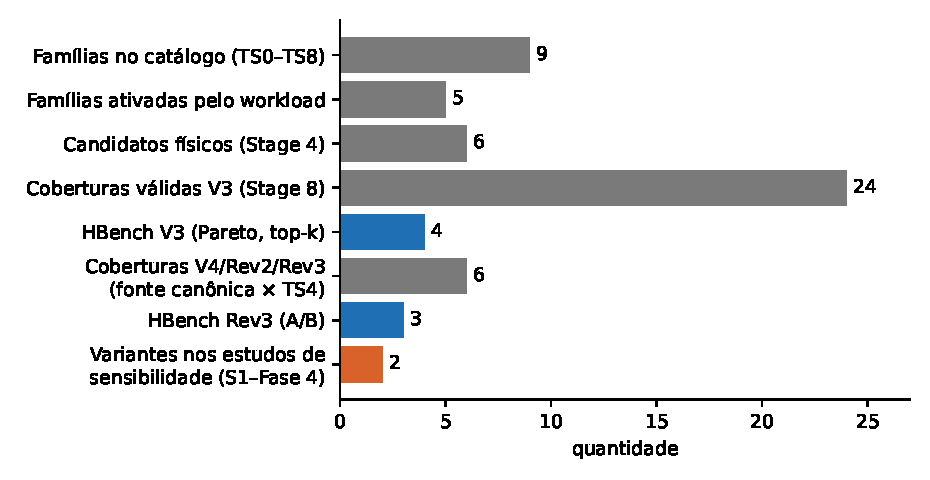
\includegraphics[width=0.85\linewidth]{figs/fig_funil.pdf}
\caption{Funil de redução do espaço de projeto ao longo das revisões. Os números vêm dos manifestos do Stage 8 (V3 nativa e Rev3 B).}
\label{fig:funil}
\end{figure}

\subsection{V3 nativa (16/10): o primeiro HBench e a primeira medição}
Dados: 3 dispositivos, 2 sensores, 1\,800 células. Das 24 coberturas válidas, o Stage 8 congelou 4: \{TS0+TS4\}, \{TS0+TS2-U+TS4\}, \{TS0+TS2-D+TS4\} e \{TS0\}. TS1 e TS5 não chegaram ao HBench (TS1 é dominada por TS2 nas mesmas consultas --- uma partição por sensor dobra as requisições ---; TS5 é condicional/inelegível).

\begin{table}[H]\centering\small
\caption{Primeiro Stage 9 (média dos 12 p95 por classe, ms). Referência = tradução do modelo \texttt{table} do IoTDB.}
\begin{tabular}{@{}lrr@{}}\toprule
Deployment & média p95 & vs.\ referência\\\midrule
Referência (\texttt{iot\_reference\_table}) & 0,681 & ---\\
TS0+TS2-D+TS4 & 1,017 & +49\%\\
TS0+TS2-U+TS4 & 1,056 & +55\%\\
TS0+TS4 & 1,351 & +98\%\\
TS0 & 1,567 & +130\%\\\bottomrule
\end{tabular}\end{table}

\textbf{Leitura:} todo o HBench foi mais lento que a referência; a única vitória foi Q8 via TS4. Esse resultado negativo motivou os diagnósticos.

\subsection{Diagnósticos E1--E3 (26/10)}
\begin{itemize}
\item \textbf{E1 (decomposição):} TS0 faz 2 requisições por consulta (uma partição por sensor) contra 1 da referência; o tempo é dominado por \emph{fetch} + decodificação no driver.
\item \textbf{E2 (TS2-U vs.\ referência com projeções idênticas, AB/BA):} empate em todas as 12 classes (TS2-U venceu entre 26 e 35 de 60 pares; deltas médios $<0{,}1$\,ms). \textbf{TS2-U e a referência são a mesma tabela.}
\item \textbf{E3 (1, 7 e 30 dias sintéticos):} sem Q8, a referência foi mais rápida em todas as escalas; a vantagem de TS4 em Q8 vinha de a referência fazer \emph{full scan} (9\,000 linhas em 30 dias) em vez de ler em ordem descendente. Na sonda Q2 de 30 dias: referência 51,0\,ms, TS2-U 48,1\,ms (1 requisição), TS2-D 74,3\,ms (30 requisições).
\end{itemize}

\just{Antes de mudar o seletor, era preciso saber se a derrota vinha do \emph{esquema}, do \emph{plano de leitura} ou do \emph{executor}. E2 e E3 mostraram que parte vinha do executor (Q8) e parte da obrigatoriedade de TS0.}

\subsection{V4 (26/10): fonte canônica selecionável e cobertura cruzada}
Duas ideias, pré-especificadas a partir de E1--E3: (i) a fonte canônica não precisa ser TS0 --- pode ser TS2-U ou TS2-D; (ii) \emph{cobertura cruzada}: uma estrutura materializada por causa de Q2 pode responder Q7 ou Q8 se o oráculo confirmar. O espaço passa a ser \{TS0, TS2-U, TS2-D\} $\times$ \{com TS4, sem TS4\} = 6 coberturas. O V4-Auto congelou TS2-U e TS2-D empatadas no Pareto (dataset de 1 dia não as distingue) e TS0 por diversidade. O controle \texttt{BASELINE\_Q8\_OPTIMIZED} (mesma tabela da referência, Q8 lida em ordem DESC parando no último valor não nulo) foi criado para isolar o efeito do plano.

\limit{Os resultados medidos da V4 (E4, 1/7/30 dias, em \texttt{outputs/diagnostics\_v4/}) são exploratórios: o desenho foi feito depois de ver E1--E3 no mesmo dataset. Não foi encontrado um relatório consolidado do E4 no repositório.}

\subsection{V4 Rev2 (26/10 -- 05/11): custos novos e o primeiro holdout}
\paragraph{Holdout Java independente.} Novas sementes (\texttt{DATA\_SEED}=19243, \texttt{QUERY\_SEED}=38421), 6 dispositivos, 300 loops, \texttt{POINT\_STEP}=10\,min, intervalo de consulta 1 dia, \texttt{GROUP\_BY}=1\,h; 18\,000 células. Duas recuperações documentadas, sem tocar em dados ou seleção: alinhamento de \texttt{GROUP\_BY\_TIME\_UNIT} no cenário analítico e substituição de um teste de contrato TS5 que pressupunha granularidade igual à do rollup.

\paragraph{Resultados confirmatórios Rev2} (2\,400 latências; média dos 12 p95): referência Q8-otimizada 2,342\,ms; TS2-U 2,673\,ms (1,897 sem Q5); TS2-D 4,036\,ms; TS0 4,515\,ms.

\paragraph{Auditoria Stage 7 $\times$ Stage 9.} 24/24 rotas instrumentadas com \texttt{MATCH} em chamadas e linhas; as 12 rotas TS0 não instrumentadas foram medidas depois (telemetria TS0) e revelaram a discrepância: Q8 em TS0 previsto com 2 linhas, observado com 3\,000.

\paragraph{E5 (controle Q8 em TS0).} Mesma tabela, dois planos: \texttt{FULL\_SCAN} p95 = 43,3\,ms (3\,000 linhas) contra \texttt{DESC\_LIMIT1} p95 = 2,03\,ms (2 linhas), 200 amostras cada, AB/BA. A diferença é \emph{do plano}, não do esquema.

\just{A auditoria preditivo-vs-observado é o teste mais forte da parte ``explicável'': se o Stage 7 diz ``D fará 42 chamadas e iterará 6\,000 linhas'', isso pode ser conferido exatamente. A divergência de Q8 em TS0 é justamente o tipo de erro que a auditoria deve encontrar --- e levou à Rev3.}

\subsection{Rev3 \emph{plan-aware} e as campanhas confirmatórias A e B (05/11)}
A Rev3 introduz um \emph{catálogo de planos executáveis} por par candidato--consulta e um despachante estrito no Stage 9 (só executa o \texttt{plan\_id} congelado). Coeficientes da Rev2 mantidos. Duas campanhas com sementes inéditas, congeladas antes de medir:

\begin{table}[H]\centering\small
\caption{Campanhas confirmatórias Rev3.}
\begin{tabular}{@{}lrr@{}}\toprule
 & A & B\\\midrule
DATA\_SEED / QUERY\_SEED & 531007 / 531013 & 531101 / 531107\\
Dispositivos, loops & 6, 300 & 9, 600\\
Células métricas & 18\,000 & 54\,000\\
Intervalo de consulta & 1 dia & 7 dias\\
Medições por Q/variante & 60 (+5 aquec.) & 60 (+5 aquec.)\\\bottomrule
\end{tabular}\end{table}

\begin{table}[H]\centering\small
\caption{HBench Rev3 (idêntico em A e B) e resultados (média dos 12 p95 por classe, ms).}
\begin{tabular}{@{}llrrr@{}}\toprule
Deployment & Motivo da seleção & escore & A & B\\\midrule
\texttt{R3H\_38939db96444} TS2-U & PARETO\_FRONT & 1,000 & 3,027 & \textbf{7,824}\\
\texttt{R3H\_934e5af2474c} TS0 & diversidade estrutural & 2,00--2,02 & 4,422 & 9,151\\
\texttt{R3H\_d2ea1974de53} TS2-D & diversidade estrutural & 1,72--2,04 & 4,418 & 11,477\\\midrule
BASELINE\_Q8\_OPTIMIZED & controle & --- & \textbf{3,012} & 7,911\\
BASELINE\_ORIGINAL & controle & --- & 3,925 & 9,867\\\bottomrule
\end{tabular}\end{table}

Previsões do Stage 7 contra contagens observadas: \textbf{36/36 MATCH} (B). SHA-256 da seleção B: \texttt{8f886938\ldots cbcb39231}.

\textbf{Leitura:} o seletor colocou em primeiro lugar o deployment que de fato venceu (ou empatou com a referência) nas duas campanhas, e ordenou corretamente TS2-U à frente de TS0 e TS2-D. TS2-U e a referência Q8-otimizada empataram (3,03 vs.\ 3,01; 7,82 vs.\ 7,91) --- o que é esperado, pois são o mesmo DDL.

% =====================================================================
\section{Por que os experimentos recentes têm só dois candidatos}
\label{sec:doiscand}
% =====================================================================

Esta é a dúvida central e a resposta é uma cadeia de eliminações, cada uma com razão registrada:

\begin{table}[H]\centering\small
\caption{Destino de cada família e motivo.}
\begin{tabularx}{\linewidth}{@{}lY@{}}\toprule
\textbf{Família} & \textbf{O que aconteceu e por quê}\\\midrule
TS3, TS6, TS7, TS8 & \textbf{Nunca ativadas}: o workload não tem âncora de dimensão, \texttt{GROUP BY} não temporal, descoberta de séries nem segmentos de modelo (Stage 1--3).\\
TS1 & Ativada, instanciada, mas \textbf{dominada} por TS2: atende às mesmas consultas, porém com uma partição por sensor (o dobro de requisições quando a consulta lê os dois sensores). Nunca entrou num HBench.\\
TS5 & Ativada por Q7/Q11, mas \textbf{inelegível}: as janelas não estão alinhadas ao rollup pré-agregado (20\,s vs.\ 1\,h no holdout), então não responde exatamente sem ler brutos.\\
TS4 & Entrou no HBench V3 (graças a Q8 com full scan). Na V4/Rev2/Rev3, com Q8 atendida por leitura descendente na própria tabela larga, \{TS2-U+TS4\} tem o mesmo custo de leitura de \{TS2-U\} e mais armazenamento/escrita (escore 1,00012 vs.\ 1,0): \textbf{analiticamente dominada}. Além disso sua manutenção não está implementada.\\
TS0 & Fora do Pareto (escore $\approx$2,0), mantida por diversidade nas campanhas A/B, onde foi a mais lenta ou empatada com TS2-D; \textbf{saiu} dos estudos de sensibilidade por não ser a questão em aberto.\\
TS2-U & \textbf{Pareto, vencedora}. Mesmo DDL da referência.\\
TS2-D & Fora do Pareto, mantida por diversidade. \textbf{Única alternativa estruturalmente distinta que ainda podia ganhar em algum regime} (partições muito grandes, janelas curtas).\\\bottomrule
\end{tabularx}\end{table}

Assim, a partir de S1 o protocolo (documento \texttt{S2\_PLANO\_PT.md} e \texttt{PROTOCOLO\_FASE2.md}) passou a estudar uma única pergunta: \emph{existe algum regime de histórico, densidade, número de dispositivos, estado físico ou cache em que o bucket diário (TS2-D) supera a tabela sem bucket (TS2-U)?} São \textbf{experimentos de sensibilidade com planos fixos}: a seleção B é congelada e não é refeita para cada cenário. A referência \texttt{BASELINE\_Q8\_OPTIMIZED} continua como controle, sabendo-se que é idêntica a TS2-U.

\caixa[warnbg]{\textbf{Interpretação honesta.} A redução a dois candidatos \emph{não} é um defeito de implementação: é a consequência correta das regras sobre um workload estreito. Mas significa que, nesta carga, a ``diversidade de esquemas'' do SchemaLens colapsou em uma única decisão binária (o modificador M1), e que o vencedor coincide com o esquema de referência óbvio. Isso limita o que se pode afirmar sobre \emph{melhoria de desempenho}; sobre \emph{explicabilidade e redução auditável}, a evidência é boa.}

% =====================================================================
\section{Experimentos de sensibilidade TS2-U $\times$ TS2-D}
% =====================================================================

Em todos: seleção B congelada, 18 casos derivados dos objetos Java de B (Q2, Q7, Q9, Q12 em janelas de 1/7/14/21 dias + controles Q5 e Q8), \texttt{page\_size}=16, 5 aquecimentos, 60 rodadas aleatorizadas, p95 por \emph{nearest rank}, oráculo em toda execução, auditoria que recalcula tudo das latências brutas. A métrica-chave é a razão $D/U = \text{p95}_{D}/\text{p95}_{U}$ ($>1$: D mais lenta).

\subsection{S1 -- varredura de janela (05/11)}
3\,240 latências (18 casos $\times$ 3 variantes $\times$ 60), 54\,000 células, 9 dispositivos, $\approx$20,8 dias de histórico. TS2-U venceu 12 de 16 comparações temporais. Q12: D/U = 0,78 (1 dia), 1,04 (7), 1,65 (14), 1,90 (21) --- em 21 dias, 2 chamadas em U contra 42 em D para as mesmas 6\,000 linhas.

\just{Variar só a janela, mantendo dados e parâmetros não temporais, isola o fan-out de buckets, que é a diferença estrutural entre U e D.}

\subsection{S2 -- densidade com histórico fixo (05/11)}
Fatores 1, 2, 4, 8$\times$ (54k a 432k células; 3\,000 a 24\,000 linhas por dispositivo) por interpolação determinística, 12 keyspaces, 216/216 validações, 12\,960 latências. TS2-U venceu 54 de 64; a mediana D/U caiu de 1,33 (1$\times$) para 1,07 (8$\times$), sem inversão.
\textbf{Descoberta:} quase todas as tabelas estavam só em memtable (SSTable = 0) durante a medição; em 8$\times$ a referência já tinha uma SSTable e U/D não --- estado físico assimétrico.

\subsection{S3 -- estado físico controlado (10/11)}
Mesmos dados e casos, keyspaces novos, \texttt{nodetool flush} antes de medir e \emph{gate}: todas as 12 tabelas com SSTable $\geq 1$ e memtable vazia. 12\,960 latências, mesma ordem aleatória do S2 (pareamento). TS2-U venceu 48 de 64; medianas D/U 1,28 $\to$ 1,10.

\begin{figure}[H]\centering
\begin{minipage}{0.49\linewidth}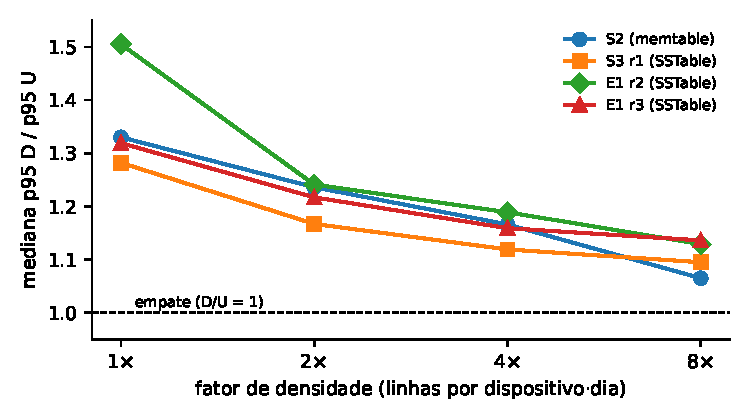
\includegraphics[width=\linewidth]{figs/fig_du_densidade.pdf}\end{minipage}\hfill
\begin{minipage}{0.49\linewidth}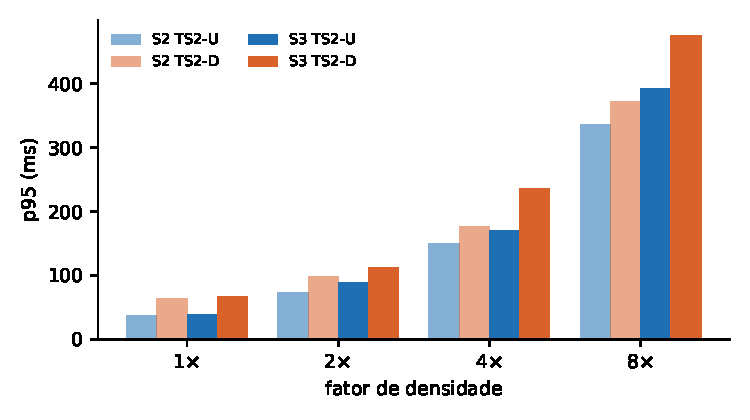
\includegraphics[width=\linewidth]{figs/fig_q12w21.pdf}\end{minipage}
\caption{Esquerda: mediana D/U nos 16 casos temporais por densidade (S2, S3 r1, E1 r2, E1 r3). Direita: Q12 em 21 dias, p95 absoluto. A penalidade relativa de D diminui com a densidade (o custo por linha passa a dominar o custo fixo por chamada), mas não se inverte.}
\end{figure}

\begin{table}[H]\centering\small
\caption{Partições medidas no S3 (\texttt{nodetool tablestats}, após flush).}
\begin{tabular}{@{}lrrr@{}}\toprule
Fator & partição média U (B) & partição média D (B) & partições U / D\\\midrule
1$\times$ & 105\,778 & 5\,662 & 9 / 189\\
8$\times$ & 943\,127 & 42\,173 & 9 / 189\\\bottomrule
\end{tabular}\end{table}

\limit{S3 $\times$ S2 mistura o efeito do flush com dia e carga do host (05/11 vs.\ 10/11); o page cache estava quente (``SSTable quente'', não disco frio). Resolvido na Fase 2 com memtable e SSTable na mesma sessão.}

\subsection{Fase 2 (E0--E6, 11/11)}
\begin{description}
\item[E1 -- réplicas r2/r3, memtable $\times$ SSTable na mesma sessão.] Em SSTable, U venceu 100 de 128 casos (r2+r3). Efeito isolado do flush em 8$\times$: REF +14,1\%, U +15,5\%, D +15,6\% --- \emph{igual para todos}, portanto não muda o vencedor. Mesmo vencedor nas três réplicas SSTable em 47/64 casos.
\item[E2 -- Rev4 (preditor log-linear).] $\ln \text{p95}=\theta_0+\theta_1\ln\text{calls}+\theta_2\ln(\text{rows}+1)+\theta_3\ln\bar{s}_{\text{part}}+\theta_4[\text{sst}]$, ajustado uma vez em 768 observações de desenvolvimento (S2, S3, E1), $R^2=0{,}985$; coeficientes: calls 0,117; rows 0,929; partição 0,014; sst 0,107. Congelado com hash antes de E3/E4.
\item[E3 -- histórico real Java (holdout).] Sementes novas, 9 dispositivos, H1 = 20,8 dias, H2 = 83,3, H3 = 333,3. Partição média de U: 103\,KB $\to$ 1\,874\,KB; mediana D/U 1,31 $\to$ 1,35. \textbf{Janelas longas (80 e 330 dias): mediana D/U = 2,06; D venceu 0 de 12.}
\item[E4 -- número de dispositivos.] N3 (D/U 1,52) e N18 (1,41): U continua vencendo.
\item[E5 -- avaliação da Rev4 no holdout.] U venceu 76/92. Acerto: Rev4 76/92 = ``sempre U'' 76/92 = ``menos chamadas'' 76/92. Erro mediano de $\ln(D/U)$: 0,138 ($\times$1,15).
\item[E6 -- cache parcialmente frio.] \texttt{posix\_fadvise(DONTNEED)} + \texttt{invalidatekeycache}: H1 D/U 1,49 $\to$ 1,47; H3 1,72 $\to$ 1,64; D venceu 3/16 e 3/24. Limitação: mmap manteve 93\% (H1) e 48\% (H3) dos bytes em cache.
\end{description}

\subsection{Fase 3 (E7--E12, 12/11)}
\begin{description}
\item[E7 -- réplicas de E3/E4.] Mesmo vencedor em 71/92; ruído típico de p95 entre réplicas: REF 5,3\%, U 5,5\%, D 8,3\%.
\item[E8 -- Rev5 (aditivo).] $\text{p95}=b_0+b_1\,\text{calls}+b_2\,\text{calls}\cdot\ln\bar{s}_{\text{part}}+b_3\,\text{rows}$, mínimos quadrados ponderados por $1/\text{p95}^2$, 752 observações. Coeficientes: $b_1=0{,}192$\,ms/chamada, $b_2=0{,}043$\,ms/(chamada$\cdot\ln$B), $b_3=0{,}0063$\,ms/linha. \emph{Leitura física:} uma chamada custa $\approx 0{,}19+0{,}043\ln(10^5)\approx 0{,}69$\,ms numa partição U de 100\,KB e $\approx0{,}56$\,ms numa partição D de 5\,KB; cada linha custa $\approx$6\,$\mu$s. Para 21 dias, D paga $\approx$20 chamadas extras $\approx$11\,ms --- é a explicação quantitativa da vitória de U.
\item[E9 -- holdout novo.] H2b (83 d), H3b (333 d), N6 (6 disp.), e \textbf{P1}: 3 dispositivos, 1 leitura/min, 333 dias, partição de U = 16,6\,MB contra 50\,KB de D. U venceu 61/80. P1: mediana D/U = 1,13; D venceu 4/20. Acerto: Rev5 59/80, Rev4 59/80, \textbf{``sempre U'' 61/80}. Erro de $\ln(D/U)$: Rev5 0,119 ($\times$1,13) contra Rev4 0,171.
\item[E10 -- tracing do servidor.] Falhou na associação por um erro de fuso horário (UTC lido como local) --- 0 de 1\,779 sessões associadas; corrigido e reassociado na Fase 4 (E13), originais preservados.
\end{description}

\begin{figure}[H]\centering
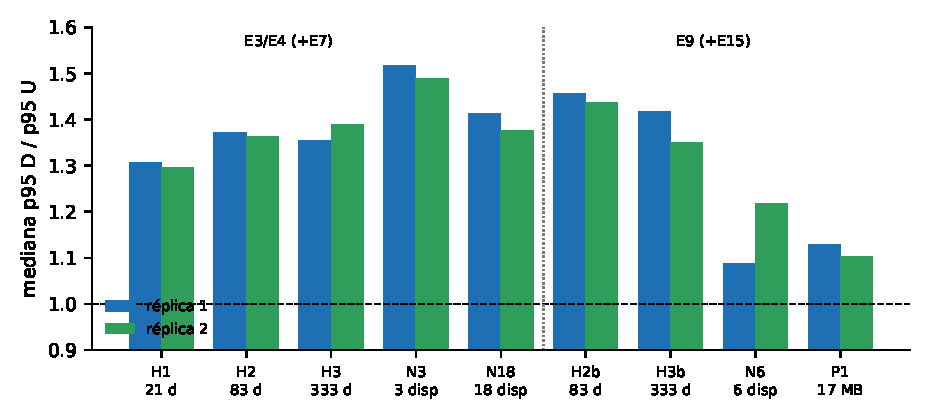
\includegraphics[width=0.85\linewidth]{figs/fig_holdout.pdf}
\caption{Mediana D/U por conjunto de holdout, duas réplicas cada. Todas acima de 1: TS2-D mais lenta em todos os cenários, inclusive com partições de 17\,MB (P1).}
\end{figure}

\subsection{Fase 4 (E13--E18, 12/11)}
\begin{description}
\item[E14 -- regra T5 com zona de empate] (congelada antes de E15): recomenda U se $\ln\hat r\geq\delta$, D se $\ln\hat r\leq-\delta$, senão ``empate técnico'' com padrão U; $\delta=0{,}10$, fixado pelo ruído entre réplicas (E7), não por E9.
\item[E15 -- réplica do holdout E9 (\texttt{e9r2}).] Mesmo vencedor em 59/80. A anomalia de P1 em janela de 1 dia (E9: D 1,7$\times$ mais lenta no p95) \textbf{não se reproduziu} (mediana 1,016).
\item[E16 -- tracing corrigido do P1.] O tempo no servidor é $\approx$25\% do tempo no cliente (ex.: Q12 7 dias, TS2-D: cliente 101\,ms, servidor 24,8\,ms em 14 requisições). O custo dominante está no driver e no processamento Python.
\item[E17 -- teste confirmatório de T5.] Rejeitada nas quatro hipóteses:
\end{description}

\begin{table}[H]\centering\small
\caption{E17 (confirmatório, \texttt{e9r2}, 80 casos temporais).}
\begin{tabular}{@{}lrrrrr@{}}\toprule
Regra & firmes & acerto firme & erros graves & arrep.\ p90 & arrep.\ máx\\\midrule
T5 & 61 & 77,0\% & 11,5\% & 0,101 & 1,50\\
Rev5 / Rev4 / menos chamadas & 80 & 77,5\% & 10,0\% & 0,099 & 1,50\\
\textbf{sempre U} & 80 & \textbf{80,0\%} & \textbf{6,3\%} & \textbf{0,075} & \textbf{0,33}\\\midrule
Hipóteses & \multicolumn{5}{l}{H5.1 graves $\leq$5\%: falhou; H5.2 acerto $\geq$90\%: falhou;}\\
 & \multicolumn{5}{l}{H5.3 arrep.\ p90 $\leq$0,10: falhou; H5.4 arrep.\ p90 $\leq$ ``sempre U'': falhou}\\\bottomrule
\end{tabular}\end{table}

\begin{figure}[H]\centering
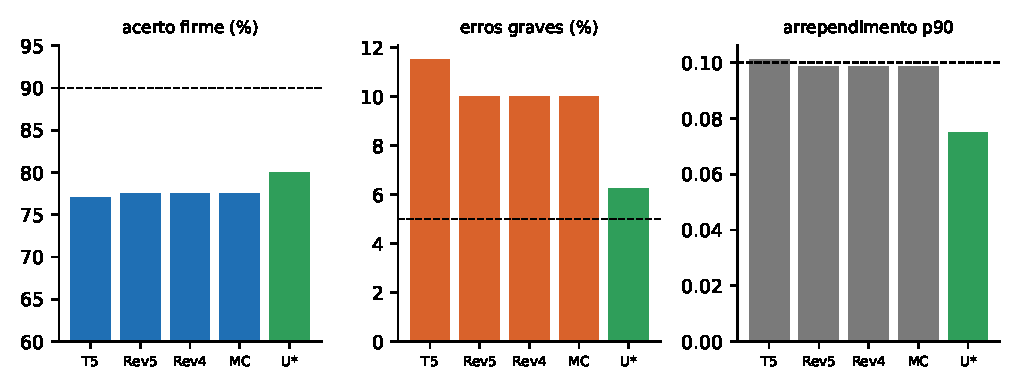
\includegraphics[width=0.9\linewidth]{figs/fig_regras.pdf}
\caption{Comparação das regras de decisão no teste confirmatório E17. Linhas tracejadas: metas pré-registradas. ``Sempre U'' (verde) é a melhor em todos os critérios; MC = ``menos chamadas vence''; U* = ``sempre U''.}
\end{figure}

\paragraph{Onde os preditores erram.} 5 dos 7 erros graves de T5 estão em janelas de 1 dia, cujas consultas levam 1--5\,ms; nesse regime o p95 de 60 amostras é dominado por pausas esporádicas, e o vencedor trocou em 10 de 16 casos entre réplicas. Ou seja: nas janelas curtas \emph{nem a medição} separa U de D --- não há o que prever.

% =====================================================================
\section{Síntese: o que está demonstrado e o que não está}
% =====================================================================

\begin{table}[H]\centering\small
\begin{tabularx}{\linewidth}{@{}YY@{}}\toprule
\textbf{Demonstrado (com evidência auditada)} & \textbf{Não demonstrado}\\\midrule
Pipeline completo, reprodutível, congelado por hash, com firewall entre seleção e medição. &
Que o SchemaLens produz um esquema \emph{mais rápido} que a referência óbvia nesta carga (o vencedor \emph{é} a referência).\\
Redução explicável: 9 famílias $\to$ 5 ativadas $\to$ 6 candidatos $\to$ 24 coberturas $\to$ 3--4 no HBench, com razão registrada para cada exclusão. &
Que a redução preserva o melhor projeto num espaço \emph{rico} (Top-$k$ preservation, regret): o espaço medido foi pequeno demais para isso.\\
Previsão estrutural exata: chamadas e linhas do Stage 7 = observado (24/24 Rev2; 36/36 Rev3 B). &
Que proxies analíticos predizem \emph{latência} melhor que uma regra trivial (Rev4, Rev5, T5 empatam ou perdem para ``sempre U'').\\
O seletor ordenou corretamente TS2-U $>$ TS0, TS2-D em dois holdouts independentes. &
Comportamento em cluster, com concorrência, escrita contínua, compactação ao longo do tempo ou cache realmente frio.\\
Robustez da escolha U: $\sim$75--80\% dos casos em 9 cenários, 2--3 réplicas, SSTable/memtable, cache quente/parcial; D nunca vence em janelas longas. &
Equivalência com o SQL oficial do IoTDB e com o mix operacional oficial.\\
Mecanismo explicativo quantificado: custo fixo por chamada ($\approx$0,6\,ms) $\times$ número de buckets. &
Que o tamanho de partição em disco seja bom preditor (coeficiente 0,014 na Rev4).\\\bottomrule
\end{tabularx}\end{table}

\subsection{Como fica a ``explicabilidade''}
Cada deployment do HBench Rev2/Rev3 tem um registro do tipo
\begin{lstlisting}
{ "deployment_id": "R2H_e72ef4d8529d", "selection_reason": "PARETO_FRONT",
  "query_id": "Q12", "plan_id": "Q12__ts2_iot_wide_unbucketed",
  "request_count_proxy": 2, "physical_rows_proxy": 2018,
  "extra_bucket_fanout_proxy": 0, "returned_bytes_proxy": 80720,
  "measured_performance_used": false }
\end{lstlisting}
A explicação ``TS2-U foi escolhida porque responde Q2/Q9/Q12 com uma chamada por dispositivo, enquanto TS2-D precisa de uma por dia; TS4 foi descartada porque a leitura descendente na tabela larga já atende Q8 sem custo de manutenção; TS5 não é exata com janelas não alinhadas'' é inteiramente derivável dos artefatos e foi confirmada pelas contagens medidas. Esse é o resultado mais sólido do projeto.

% =====================================================================
\section{Leitura crítica}
% =====================================================================
\begin{enumerate}
\item \textbf{O workload determinou o resultado.} Com um dispositivo e dois sensores DOUBLE por consulta, a tabela larga por dispositivo é quase obrigatoriamente ótima; o IoTDB \texttt{table} já é esse projeto. O SchemaLens chegou a ele por um caminho explicável, mas não tinha espaço para fazer melhor.
\item \textbf{M1 foi explorado em só dois pontos} (dia e ``infinito''). Buckets semanais/mensais, ou bucket dimensionado pelo volume, nunca foram instanciados --- e são justamente o meio-termo que poderia vencer quando partições crescem.
\item \textbf{Armazenamento e escrita quase não pesam} (0,1 + 0,1 no escore V3; proxies de escrita idênticos entre U e D). A metodologia é multiobjetivo, mas os experimentos foram só de leitura.
\item \textbf{Muitas decisões foram motivadas por resultados anteriores} (Rev2 após o Piloto 1; V4 após E1--E3; Rev3 após E5). Isso foi tratado corretamente --- cada revisão foi testada em dados novos ---, mas deve ser declarado no texto como desenvolvimento iterativo com holdouts, não como método fixado \emph{a priori}.
\item \textbf{A métrica p95 de 60 amostras é instável em consultas de 1--5\,ms}, o que contaminou a avaliação dos preditores nas janelas curtas.
\item \textbf{A latência é do cliente Python}; o servidor responde por $\approx$25\% do tempo (E16). Diferenças de esquema aparecem diluídas pelo custo do driver.
\end{enumerate}

% =====================================================================
\section{O que pode ser concluído agora}
% =====================================================================
\begin{enumerate}
\item \textbf{Conclusão metodológica:} o SchemaLens adaptado ao Cassandra/TSDB produz uma redução do espaço de projeto \emph{rastreável regra a regra}, com congelamento verificável e previsão estrutural exata do trabalho de cada consulta; a ordenação pré-benchmark coincidiu com a ordenação medida em dois holdouts independentes.
\item \textbf{Conclusão de engenharia (para este workload):} sem bucket (TS2-U) é a escolha correta para leituras por dispositivo em janelas de até 333 dias e partições de até $\approx$17\,MB, num nó; o bucket diário custa uma chamada por dia e perde de forma crescente com a janela (D/U $\approx$2 em 80--330 dias). O efeito do estado físico (flush) e do cache parcial é o mesmo para as duas variantes.
\item \textbf{Resultado negativo pré-registrado:} preditores de latência baseados nos proxies (Rev4, Rev5) e a regra com zona de empate T5 não superam ``sempre U''. Isso reforça a credibilidade do protocolo e indica que o valor do SchemaLens está na \emph{seleção estrutural}, não na regressão de latência.
\item \textbf{Limite da afirmação:} não afirmar ganho de desempenho sobre a referência, nem generalização para cluster, concorrência ou outros workloads.
\end{enumerate}

% =====================================================================
\section{O que pode (e deveria) ser ajustado}
% =====================================================================

\begin{longtable}{@{}p{0.4cm}p{5.2cm}p{6.3cm}p{1.8cm}@{}}
\toprule
\# & \textbf{Ajuste} & \textbf{Por quê / o que responde} & \textbf{Custo}\\\midrule\endhead
1 & \textbf{Ampliar o workload para ativar mais famílias}: consultas multi-dispositivo e por dimensão (tags, região/tipo), \texttt{GROUP BY} não temporal, alta frequência de ``último valor'', agregações em janelas alinhadas; \texttt{QUERY\_DEVICE\_NUM}$>1$, \texttt{QUERY\_SENSOR\_NUM} $<$ número de sensores. & É a única forma de testar a tese central (``gerar esquemas diferentes e melhores''): ativaria TS3, TS4 (com manutenção), TS5, TS6, TS7 e criaria trade-offs reais em que a referência não é ótima. & alto\\
2 & \textbf{Explorar M1 em mais pontos}: TS2 com bucket de hora, semana, mês e bucket dimensionado pelo volume esperado. & Hoje a decisão de granularidade é binária; o meio-termo pode vencer U em partições grandes sem pagar o fan-out diário. & médio\\
3 & \textbf{Muitos sensores e sensores esparsos/heterogêneos} (\texttt{SENSOR\_NUMBER} 10--100, \texttt{NULL\_RATIO}$>0$, tipos não DOUBLE) com consultas que projetam subconjuntos. & Cria o trade-off TS0 (estreita) $\times$ TS2 (larga) que hoje não existe com 2 sensores. & médio\\
4 & \textbf{Usar \texttt{OPERATION\_PROPORTION}} para pesar consultas (em vez de frequência uniforme) e medir p95 do mix. & Aproxima o escore do uso real e da métrica oficial. & baixo--médio\\
5 & \textbf{Incluir escrita e manutenção}: ingestão contínua, TS4/TS5 mantidas, compactação ao longo do tempo, bytes reais de SSTable. & Dá peso real aos objetivos de armazenamento/escrita do Pareto. & médio\\
6 & \textbf{Política de medição para consultas curtas} (EMENDA\_06): mais amostras, mediana + p95 com IC por \emph{bootstrap}~\cite{efron}, testável primeiro nas latências brutas já gravadas. & Evita que o ruído de 1--5\,ms decida vencedores e preditores. & baixo\\
7 & \textbf{Partições grandes com mais dispositivos} (P2: 9--18 disp., $\sim$17\,MB). & Única combinação ainda não testada em que D poderia vencer com folga. & médio--alto\\
8 & \textbf{Cache frio real} (reinício do container + limpeza do page cache do host). & E6 só obteve cache parcialmente frio (mmap). Requer autorização. & médio\\
9 & \textbf{Cluster de 3+ nós e clientes concorrentes} (ou \texttt{cassandra-stress}/cliente Java). & Partições grandes e fan-out se comportam diferente com rede, coordenação e hot spots (M4). & alto\\
10 & \textbf{Comparação com outros métodos de projeto} (Chebotko~\cite{chebotko2015}, NoSE~\cite{nose}) no mesmo workload. & Posiciona o SchemaLens na literatura. & médio\\
11 & \textbf{Rev6} só se o artigo quiser defender um preditor: corrigir o viés de 1 dia, calibrar em E9+e9r2, testar em holdout inédito. & Única forma honesta de recuperar uma regra preditiva. & médio\\
12 & \textbf{Manutenção}: limpar keyspaces \texttt{sl\_f2\_*}, \texttt{sl\_s2\_*}, \texttt{sl\_s3\_*} (irreversível; evidências já zipadas); unificar READMEs num índice. & Memória/disco e legibilidade do repositório. & baixo\\
\bottomrule
\end{longtable}

\paragraph{Recomendação de ordem.} (a) Escrever o artigo com o enquadramento ``redução explicável e auditável + resultado negativo dos preditores'', usando os resultados das Fases 2--4 como estão; (b) fazer o item 6 (barato, melhora a análise já feita); (c) se o objetivo for demonstrar \emph{ganho de desempenho} --- que é a promessa original --- priorizar os itens 1--3, porque sem um workload mais rico o SchemaLens não tem o que melhorar sobre a referência.

% =====================================================================
\section{Ameaças à validade}
% =====================================================================
\begin{itemize}
\item \textbf{Interna:} nó único compartilhado com outros containers; tempo no cliente Python; p95 de 60 amostras dependentes; múltiplas comparações sem correção; dados de S2/S3/E1 densificados sinteticamente.
\item \textbf{Construto:} \texttt{execute\_calls} e \texttt{iterated\_rows} são do cliente, não I/O do servidor; ``média dos p95 por classe'' não é o p95 do mix.
\item \textbf{Externa:} uma família de workloads (IoT Benchmark, modo \texttt{table}, 2 sensores DOUBLE); planos fixos da seleção B nos estudos de sensibilidade; Cassandra 4.1.12.
\item \textbf{Conclusão:} desenvolvimento iterativo (cada revisão motivada por resultados anteriores), mitigado por holdouts com sementes Java inéditas e pré-registro.
\end{itemize}

% =====================================================================
\appendix
\section{Mapa de artefatos}
\begin{longtable}{@{}p{5.5cm}p{9cm}@{}}\toprule
\textbf{Artefato} & \textbf{Conteúdo}\\\midrule\endhead
\texttt{phase\_a1/vendor/tsdb\_base/config/} & catálogo TS0--TS8, regras de ativação e de modificadores (com hash)\\
\texttt{iot\_pipeline/stage4.py}\,\ldots\,\texttt{stage9.py} & Stages 4--9 da V3\\
\texttt{config/pipeline\_policy.json} & pesos V3, fatores de família, \texttt{top\_k}, variantes TS2\\
\texttt{native\_auto\_work/runs/v3\_20261016T191603Z\_*} & V3 nativa, Stage 9, E1--E3, V4, V4-Auto\\
\texttt{SchemaLens\_V4\_Rev2\_Confirmatory/} & custos Rev2, holdout Java, executor confirmatório\\
\texttt{SchemaLens\_V4\_Rev3\_PlanAware/} & catálogo de planos executáveis, despachante estrito\\
\texttt{rev3\_confirmatory\_\{A,B\}\_results.zip} & HBench Rev3, latências, \texttt{stage7\_vs\_stage9.csv}\\
\texttt{experiments/rev3\_s2\_partition\_growth/} & S1 (casos), S2\\
\texttt{experiments/rev3\_s3\_physical\_storage/} & S3 R1, \texttt{FINAL\_AUDIT\_PT.md}\\
\texttt{experiments/rev3\_fase2/} & protocolo, EMENDA\_01--05, E1--E18, Rev4, Rev5, \texttt{analysis/*.json}\\
\texttt{SchemaLens\_Rev3\_Fase3\_Fase4\_results.zip} & 912 arquivos, SHA-256 \texttt{73437491cdfd07e5\ldots}\\\bottomrule
\end{longtable}

\section{Glossário rápido}
\begin{description}
\item[HBench] conjunto congelado de deployments a medir. \textbf{Deployment}: combinação de tabelas + rota por consulta.
\item[TS2-U / TS2-D] tabela larga sem bucket / com bucket diário. \textbf{REF}: tradução Cassandra do modelo \texttt{table} do IoTDB (mesmo DDL de TS2-U).
\item[D/U] razão p95 de TS2-D sobre p95 de TS2-U no mesmo caso.
\item[Fan-out] número de partições (buckets) que uma consulta precisa tocar.
\item[Memtable / SSTable] estrutura em memória / arquivo imutável em disco na árvore LSM do Cassandra~\cite{lakshman,lsm}.
\item[Arrependimento] $\ln(\text{p95 da variante recomendada}/\min(\text{p95}_U,\text{p95}_D))$.
\end{description}

\begin{thebibliography}{99}\small
\bibitem{chebotko2015} A.~Chebotko, A.~Kashlev, S.~Lu. A Big Data Modeling Methodology for Apache Cassandra. \emph{IEEE International Congress on Big Data}, 2015.
\bibitem{nose} M.~J.~Mior, K.~Salem, A.~Aboulnaga, R.~Liu. NoSE: Schema Design for NoSQL Applications. \emph{IEEE ICDE}, 2016; versão estendida em \emph{IEEE TKDE}, 2017.
\bibitem{lakshman} A.~Lakshman, P.~Malik. Cassandra: a decentralized structured storage system. \emph{ACM SIGOPS Operating Systems Review}, 44(2), 2010.
\bibitem{lsm} P.~O'Neil, E.~Cheng, D.~Gawlick, E.~O'Neil. The log-structured merge-tree (LSM-tree). \emph{Acta Informatica}, 33(4), 1996.
\bibitem{modelardb} S.~K.~Jensen, T.~B.~Pedersen, C.~Thomsen. ModelarDB: Modular Model-Based Time Series Management with Spark and Cassandra. \emph{PVLDB}, 11(11), 2018.
\bibitem{iotbench} thulab/iot-benchmark. \url{https://github.com/thulab/iot-benchmark}, commit \texttt{62e0dc100e56443978c8b4c66472b1d8a7ef0238}.
\bibitem{iotbenchpaper} R.~Liu, J.~Yuan et al. Benchmarking Time Series Databases with IoTDB-Benchmark for IoT Scenarios. arXiv:1901.08304, 2019.
\bibitem{nosek2018} B.~A.~Nosek, C.~R.~Ebersole, A.~C.~DeHaven, D.~T.~Mellor. The preregistration revolution. \emph{PNAS}, 115(11), 2018.
\bibitem{hyndman} R.~J.~Hyndman, Y.~Fan. Sample quantiles in statistical packages. \emph{The American Statistician}, 50(4), 1996.
\bibitem{ehrgott} M.~Ehrgott. \emph{Multicriteria Optimization}. 2.ª ed., Springer, 2005.
\bibitem{efron} B.~Efron, R.~J.~Tibshirani. \emph{An Introduction to the Bootstrap}. Chapman \& Hall, 1993.
\end{thebibliography}

\end{document}
